\chapter{Evaluation}

\section{Introduction}
This chapter will present the results of this research. First, the evaluation metrics that were used to evaluate the classifiers will be introduced. The results of the evaluation of the thirteen classifiers with the seven different feature representations will be outlined. The methods used to evaluate the recommender system will be defined. Finally, the results of this evaluation will be presented. 

\section{Evaluation Metrics for Classification}

\subsection{Confusion Matrix}
A confusion matrix is a technique commonly used for evaluating the performance of a classification model. It presents a summary of the prediction results of the classifier. A confusion matrix consists of four different combinations of the actual values versus the predicted values. 

\begin{table}[h!]
\setlength\extrarowheight{5pt}
\caption{Confusion Matrix.}
\label{Table:confusionmatrix}
\begin{tabular}{c|c|c|}
\cline{2-3}
 & \multicolumn{1}{l|}{Actual Positive} & \multicolumn{1}{l|}{Actual Negative} \\ \hline
\multicolumn{1}{|l|}{Predicted Positive} & TP & FP \\ \hline
\multicolumn{1}{|l|}{Predicted Negative} & FN & TN \\ \hline
\end{tabular}
\end{table}

The values in a confusion matrix are:
\begin{itemize}
    \item \textbf{True Positive (TP)}\newline
    You have a True Positive value if your algorithm classified an item as positive and this was correct.
    \item \textbf{False Positive (FP)}\newline
    You have a False Positive value if your algorithm classified an item as positive but the value was actually negative.
    \item \textbf{False Negative (FN)}\newline
    You have a False Negative value if your algorithm classified an item as negative but the value was actually positive.
    \item \textbf{True Negative (TN)}\newline
    You have a True Negative value if your algorithm classified an item as negative and this was correct.
\end{itemize}

The confusion matrix is useful for calculating the precision, recall, accuracy and f1-score of a classification algorithm. These four metrics were used to evaluate the performance of the classifiers.

\subsection{Precision}
Precision is the percentage of positive identifications that were classified correctly.
\begin{equation}
    Precision\ =\ \cfrac{True\ Positives}{True\ Positives\ +\ False\ Positives}
\end{equation}
The higher the precision score the better. A low precision score can indicate that there is a large number of false positives. A high precision score indicates that the majority of what was classified, was classified correctly. You could however, have a very high precision in the case where only a small portion of samples were actually classified but of these the majority were classified correctly. In this case the precision is high but the recall would be very low.

\subsection{Recall}
Recall is the percentage of all actual positives that were classified correctly.
\begin{equation}
    Recall\ =\ \cfrac{True\ Positives}{True\ Positives\ +\ False\ Negatives}
\end{equation}
The higher the recall score the better. A low recall value can indicate there are a large number of false negatives. A high recall value indicates that the majority of what should have been classified as a was classified correctly. You could however have a very high recall and low precision if everything was classified. All the samples that that should have been classified are classified correctly, giving the high recall. But a lot of extra samples are classified that shouldn't have been classified, giving a low precision.

\subsection{Accuracy}
Accuracy is the total number of predictions the classifier got right. It is the percentage of the tweets that were classified correctly.
\begin{equation}
    Accuracy\ =\ \cfrac{Number\ of\ Correct\ Predictions}{Total\ Number\ of\ Predictions}
\end{equation}
The higher the accuracy score the better, but a high accuracy does not always give an accurate representation of the situation if there is a major class imbalance.

\subsection{F1-Score}
F1-Score is the harmonic mean of precision and recall. It is also called the F-Score or F-Measure. 
\begin{equation}
    F1-Score\ =\ 2 \times\ \cfrac{Precision\ \times\ Recall}{Precision\ +\ Recall}
\end{equation}
The higher the F1-Score the better. A high F1-Score indicates a good balance between precision and recall.

\subsection{Multi-Class Classification}
Multi-Class Classification is any classification task that involves two or more classes. This research tackles a multi-class classification problem. We aim to classifying tweets as one of the following three classes: 'review', 'some content', or 'irrelevant'. For a binary classification problem, the precision, recall, f1-score and accuracy scores can be calculated simply with the above formulas. For multi-class classification there needs to be a way of getting an average metric over the three classes, rather than an individual class score.
There are three ways that precision, recall, f1-score and accuracy can be calculated for this kind of multi-class classification problem:
\begin{enumerate}
    \item \textbf{Micro Average:}\newline
    The micro average calculates the metrics globally. It aggregates the contributions of all classes, counting the total true positives, false negatives and false positives, to calculate the overall average scores.  
    \item \textbf{Macro Average:}\newline
    The macro average calculates the metrics independently for each class. It then calculates the unweighted mean of the scores of the three classes.
    \item \textbf{Weighted Average:}\newline
    The weighted average calculates the metrics independently for each class, like the macro average does. It then calculates the weighted average of the scores of the three classes. This differs from macro average in that it takes class imbalance into account.
\end{enumerate}

The metrics listed in the tables below (Tables ~\ref{Table:precision},~\ref{Table:recall},~\ref{Table:accuracy},~\ref{Table:f1score}) were calculated with the weighted average.

\section{Classification Results and Analysis}

In this section, the results and evaluation of the classifiers will be presented. The classifiers evaluated include:
\begin{enumerate}
    \item Random Forest (RF) Classifier.
    \item Decision Tree (DT) Classifier.
    \item Multi Layer Perceptron (MLP) Classifier.
    \item Support Vector Machine (SVM) Classifier.
    \item Logistic Regression (LR) Classifier.
    \item K Nearest Neighbours (KNN) Classifier.
    \item Gaussian Process (GP) Classifier.
    \item AdaBoost (AB) Classifier.
    \item Gaussian Naïve Bayes (GNB) Classifier.
    \item Multinomial Naïve Bayes (MNB) Classifier.
    \item Bernouilli Naïve Bayes (BNB) Classifier.
    \item Quadratic Discriminant Analysis (QDA) Classifier.
    \item Linear Discriminant Analysis (LDA) Classifier.
\end{enumerate}

These classifiers were evaluated with seven different feature representations defined below:
\begin{enumerate}
    \item Unigram Bag-of-Words (BOW).
    \item Unigram TF-IDF.
    \item Bigram TF-IDF.
    \item Trigram TF-IDF.
    \item Unigram TF-IDF with stop words removed.
    \item Doc2Vec.
    \item Word2Vec.
\end{enumerate}

Taking the thirteen classifiers and seven feature representations there are 91 different combinations. Each was evaluated in terms of precision, recall, accuracy and f1-score.

The set of 3115 tweets was divided into a training set and a testing set with a 80:20 split. The label distribution of the data is shown in the table below (Table ~\ref{Table:tweetlabels}).

\begin{table}[h!]
\setlength\extrarowheight{5pt}
\caption{Distribution of Tweet Labels.}
\label{Table:tweetlabels}
\begin{tabular}{|c|c|}
\hline
\textbf{Label} & \textbf{Tweet Count} \\ \hline
Review         & 566                  \\ \hline
Some Content   & 910                  \\ \hline
Irrelevant     & 1639                 \\ \hline
\end{tabular}
\end{table}

\subsection{Precision}

\begin{table}[h!]
\setlength\extrarowheight{5pt}
\caption{Precision of Classifiers for different Feature Representations.}
\label{Table:precision}
\resizebox{\textwidth}{!}{
\begin{tabular}{cccccccc}
\specialrule{1.5pt}{1pt}{1pt}
 & \textbf{BOW} & \textbf{\begin{tabular}[c]{@{}c@{}}TF-IDF\\ (Unigram)\end{tabular}} & \textbf{\begin{tabular}[c]{@{}c@{}}TF-IDF\\ (Bigram)\end{tabular}} & \textbf{\begin{tabular}[c]{@{}c@{}}TF-IDF\\ (Trigram)\end{tabular}} & \textbf{\begin{tabular}[c]{@{}c@{}}TF-IDF\\ (Unigram,\\ No Stop Words)\end{tabular}} & \textbf{Doc2Vec} & \textbf{Word2Vec} \\ \specialrule{1.5pt}{1pt}{1pt}
\textbf{RF} & 0.72 & 0.74 & 0.7 & 0.69 & 0.73 & 0.59 & 0.71 \\ \hline
\rowcolor[HTML]{EFEFEF} 
\textbf{DT} & 0.57 & 0.58 & 0.58 & 0.59 & 0.63 & 0.56 & 0.54 \\ \hline
\textbf{MLP} & 0.71 & 0.71 & 0.7 & 0.7 & 0.7 & 0.59 & 0.71 \\ \hline
\rowcolor[HTML]{EFEFEF} 
\textbf{SVM} & 0.56 & 0.74 & 0.73 & 0.71 & 0.71 & 0.62 & 0.71 \\ \hline
\textbf{LR} & 0.72 & 0.72 & 0.7 & 0.68 & 0.7 & 0.61 & 0.71 \\ \hline
\rowcolor[HTML]{EFEFEF} 
\textbf{KNN} & 0.53 & 0.62 & 0.62 & 0.62 & 0.61 & 0.54 & 0.67 \\ \hline
\textbf{GP} & 0.72 & 0.72 & 0.71 & 0.69 & 0.7 & 0.61 & 0.72 \\ \hline
\rowcolor[HTML]{EFEFEF} 
\textbf{AB} & 0.63 & 0.62 & 0.63 & 0.62 & 0.64 & 0.57 & 0.63 \\ \hline
\textbf{GNB} & 0.6 & 0.6 & 0.63 & 0.63 & 0.59 & 0.59 & 0.64 \\ \hline
\rowcolor[HTML]{EFEFEF} 
\textbf{MNB} & \multicolumn{1}{c}{\cellcolor[HTML]{EFEFEF}0.71} & 0.67 & 0.68 & 0.66 & 0.67 &  &  \\ \hline
\rowcolor[HTML]{FFFFFF} 
\textbf{BNB} & 0.73 & 0.73 & 0.71 & 0.71 & 0.72 & 0.58 & 0.65 \\ \hline
\rowcolor[HTML]{EFEFEF} 
\textbf{QDA} & 0.72 & 0.76 & 0.73 & 0.67 & \textcolor{red}{0.79} & 0.57 & 0.59 \\ \hline
\rowcolor[HTML]{FFFFFF} 
\textbf{LDA} & 0.63 & 0.64 & 0.65 & 0.63 & 0.62 & 0.66 & 0.69 \\ \hline
\end{tabular}}
\end{table}

In terms of precision, the QDA classifier with unigram TF-IDF and no stop words feature representation was the best performing classifier achieving a precision score of 0.79 (Table ~\ref{Table:precision}). This indicates that the QDA classifier had a high percentage of positive identifications that were classified correctly. The QDA classifier with unigram TF-IDF feature representation, this time with stop words included achieved the next highest precision score of 0.76. This further confirmed that unigram feature representation seems to work best with the QDA classifier. The RF classifier and the SVM classifier, both with unigram TF-IDF feature representation were the two next best performing classifiers both achieving precision values of 0.74.

It is interesting to compare our precision scores to those in the study by A.Rane and A.Kumar \cite{Rane2018}, in which they investigated the performance of various classifiers in classifying the sentiment of Twitter reviews about airlines. They found that the RF classifier achieved the highest precision score, followed first by AdaBoost and then the SVM classifier. They did not include the QDA classifier in their evaluation. Our results do not fully confirm or contradict the results of A.Rane and A.Kumar \cite{Rane2018}. Two out of three of our top performing classifiers agree, the RF classifier and the SVM classifier. Their precision scores are higher than ours for all the classifiers that they implemented, at approximately 0.8 compared to ours at approximately 0.7. A likely reason for this is that they trained their classifiers on a much larger dataset, a total of 14640 tweets, while our classifiers were trained on a smaller set of 3116 tweets. Supervised machine learning methods tend to perform the best on large datasets. Our results could possibly be improved by collecting and annotating a larger dataset.

\subsection{Recall}

\begin{table}[h!]
\setlength\extrarowheight{5pt}
\caption{Recall of Classifiers for different Feature Representations.}
\label{Table:recall}
\resizebox{\textwidth}{!}{
\begin{tabular}{cccccccc}
\specialrule{1.5pt}{1pt}{1pt}
 & \textbf{BOW} & \textbf{\begin{tabular}[c]{@{}c@{}}TF-IDF\\ (Unigram)\end{tabular}} & \textbf{\begin{tabular}[c]{@{}c@{}}TF-IDF\\ (Bigram)\end{tabular}} & \textbf{\begin{tabular}[c]{@{}c@{}}TF-IDF\\ (Trigram)\end{tabular}} & \textbf{\begin{tabular}[c]{@{}c@{}}TF-IDF\\ (Unigram,\\ No Stop Words)\end{tabular}} & \textbf{Doc2Vec} & \textbf{Word2Vec} \\ \specialrule{1.5pt}{1pt}{1pt}
\textbf{RF} & 0.7 & 0.71 & 0.7 & 0.69 & 0.72 & 0.64 & 0.69 \\ \hline
\rowcolor[HTML]{EFEFEF} 
\textbf{DT} & 0.61 & 0.6 & 0.61 & 0.62 & 0.65 & 0.59 & 0.56 \\ \hline
\textbf{MLP} & 0.72 & 0.72 & 0.71 & 0.71 & 0.71 & 0.62 & 0.72 \\ \hline
\rowcolor[HTML]{EFEFEF} 
\textbf{SVM} & 0.59 & \textcolor{red}{0.74} & \textcolor{red}{0.74} & 0.72 & 0.72 & 0.64 & 0.72 \\ \hline
\textbf{LR} & 0.72 & 0.72 & 0.71 & 0.7 & 0.71 & 0.64 & 0.72 \\ \hline
\rowcolor[HTML]{EFEFEF} 
\textbf{KNN} & 0.61 & 0.66 & 0.66 & 0.65 & 0.65 & 0.61 & 0.68 \\ \hline
\textbf{GP} & 0.73 & 0.73 & 0.72 & 0.71 & 0.71 & 0.64 & 0.73 \\ \hline
\rowcolor[HTML]{EFEFEF} 
\textbf{AB} & 0.65 & 0.64 & 0.65 & 0.65 & 0.66 & 0.61 & 0.64 \\ \hline
\textbf{GNB} & 0.48 & 0.48 & 0.47 & 0.45 & 0.48 & 0.49 & 0.56 \\ \hline
\rowcolor[HTML]{EFEFEF} 
\textbf{MNB} & \multicolumn{1}{c}{\cellcolor[HTML]{EFEFEF}0.66} & 0.68 & 0.69 & 0.67 & 0.68 &  &  \\ \hline
\rowcolor[HTML]{FFFFFF} 
\textbf{BNB} & 0.71 & 0.71 & 0.66 & 0.62 & 0.71 & 0.54 & 0.56 \\ \hline
\rowcolor[HTML]{EFEFEF} 
\textbf{QDA} & 0.26 & 0.23 & 0.24 & 0.56 & 0.26 & 0.68 & 0.61 \\ \hline
\rowcolor[HTML]{FFFFFF} 
\textbf{LDA} & 0.61 & 0.61 & 0.61 & 0.59 & 0.59 & 0.67 & 0.69 \\ \hline
\end{tabular}}
\end{table}

The SVM classifier was the best performing classifier with regard to recall, achieving a recall score of 0.74 (Table ~\ref{Table:recall}). The unigram TF-IDF and bigram TF-IDF feature representations performed equally well. This again partly agrees with \cite{Rane2018}, who found that the SVM classifier was their second best performing classifier in terms of recall, with the RF classifier again coming out on top. Our scores are again slightly lower than those of A.Rane and A.Kumar.

Notice that the QDA classifier which performed the best in precision, performs pretty poorly in terms of recall. This is a common issue and is why we have also evaluated the classifiers with the f1-score. The f1-score conveys the balance between precision and recall giving us a better idea of the actual performance of the classifier.

The GP classifier was the next highest performing classifier, achieving a recall score of 0.73, with unigram TF-IDF feature representation. This is interesting as I have not come across any studies where a GP classifier has been applied to tweets. The GP classifier also performed well in precision achieving a precision score of 0.72.  

\subsection{F1-Score}

\begin{table}[h!]
\setlength\extrarowheight{5pt}
\caption{F1-Score of Classifiers for different Feature Representations.}
\label{Table:f1score}
\resizebox{\textwidth}{!}{
\begin{tabular}{cccccccc}
\specialrule{1.5pt}{1pt}{1pt}
 & \textbf{BOW} & \textbf{\begin{tabular}[c]{@{}c@{}}TF-IDF\\ (Unigram)\end{tabular}} & \textbf{\begin{tabular}[c]{@{}c@{}}TF-IDF\\ (Bigram)\end{tabular}} & \textbf{\begin{tabular}[c]{@{}c@{}}TF-IDF\\ (Trigram)\end{tabular}} & \textbf{\begin{tabular}[c]{@{}c@{}}TF-IDF\\ (Unigram,\\ No Stop Words)\end{tabular}} & \textbf{Doc2Vec} & \textbf{Word2Vec} \\ \specialrule{1.5pt}{1pt}{1pt}
\textbf{RF} & 0.65 & 0.65 & 0.64 & 0.64 & 0.69 & 0.59 & 0.63 \\ \hline
\rowcolor[HTML]{EFEFEF} 
\textbf{DT} & 0.57 & 0.59 & 0.58 & 0.6 & 0.63 & 0.56 & 0.54 \\ \hline
\textbf{MLP} & 0.71 & 0.7 & 0.69 & 0.69 & 0.69 & 0.57 & 0.71 \\ \hline
\rowcolor[HTML]{EFEFEF} 
\textbf{SVM} & 0.45 & \textcolor{red}{0.73} & \textcolor{red}{0.73} & 0.71 & 0.71 & 0.63 & 0.71 \\ \hline
\textbf{LR} & 0.71 & 0.7 & 0.69 & 0.68 & 0.69 & 0.6 & 0.71 \\ \hline
\rowcolor[HTML]{EFEFEF} 
\textbf{KNN} & 0.49 & 0.62 & 0.62 & 0.62 & 0.61 & 0.55 & 0.67 \\ \hline
\textbf{GP} & 0.71 & 0.71 & 0.72 & 0.7 & 0.7 & 0.61 & 0.72 \\ \hline
\rowcolor[HTML]{EFEFEF} 
\textbf{AB} & 0.63 & 0.62 & 0.63 & 0.62 & 0.63 & 0.59 & 0.63 \\ \hline
\textbf{GNB} & 0.5 & 0.51 & 0.49 & 0.47 & 0.5 & 0.51 & 0.58 \\ \hline
\rowcolor[HTML]{EFEFEF} 
\textbf{MNB} & \multicolumn{1}{c}{\cellcolor[HTML]{EFEFEF}0.67} & 0.63 & 0.66 & 0.65 & 0.64 &  &  \\ \hline
\rowcolor[HTML]{FFFFFF} 
\textbf{BNB} & 0.72 & 0.72 & 0.67 & 0.64 & 0.71 & 0.55 & 0.58 \\ \hline
\rowcolor[HTML]{EFEFEF} 
\textbf{QDA} & 0.23 & 0.19 & 0.19 & 0.48 & 0.23 & 0.61 & 0.55 \\ \hline
\rowcolor[HTML]{FFFFFF} 
\textbf{LDA} & 0.62 & 0.62 & 0.62 & 0.6 & 0.6 & 0.66 & 0.69 \\ \hline
\end{tabular}}
\end{table}

Again, the SVM classifier achieved the highest f1-score of 0.73 (Table ~\ref{Table:f1score}), with the unigram and bigram TF-IDF feature representations again performing equally well. This high f1-score indicates that the SVM classifier has a good balance of precision and recall. This confirms the results of both Rathi et al. \cite{Raithi2018}, and Rane & Kumar \cite{Rane2018} who both found in their studies that the SVM classifier performed well in classifying tweets. However, it contradicts the results of Bermingham & Smeaton who found that MNB performed better than SVM on tweets and short reviews. In our experiments SVM outperformed MNB in all metrics.

The next best performing classifiers were GP and BNB, with f1-scores of 0.72. This somewhat agrees with Bermingham & Smeaton, who found that MNB achieved the best classification results on their set of tweets. I have not come across any example of GP performing well for tweet classification.

\subsection{Accuracy}

\begin{table}[h!]
\setlength\extrarowheight{5pt}
\caption{Accuracy of Classifiers for different Feature Representations.}
\label{Table:accuracy}
\resizebox{\textwidth}{!}{
\begin{tabular}{cccccccc}
\specialrule{1.5pt}{1pt}{1pt}
 & \textbf{BOW} & \textbf{\begin{tabular}[c]{@{}c@{}}TF-IDF\\ (Unigram)\end{tabular}} & \textbf{\begin{tabular}[c]{@{}c@{}}TF-IDF\\ (Bigram)\end{tabular}} & \textbf{\begin{tabular}[c]{@{}c@{}}TF-IDF\\ (Trigram)\end{tabular}} & \textbf{\begin{tabular}[c]{@{}c@{}}TF-IDF\\ (Unigram,\\ No Stop Words)\end{tabular}} & \textbf{Doc2Vec} & \textbf{Word2Vec} \\ \specialrule{1.5pt}{1pt}{1pt}
\textbf{RF} & 0.703 & 0.706 & 0.696 & 0.691 & 0.721 & 0.635 & 0.677 \\ \hline
\rowcolor[HTML]{EFEFEF} 
\textbf{DT} & 0.614 & 0.596 & 0.614 & 0.621 & 0.652 & 0.594 & 0.563 \\ \hline
\textbf{MLP} & 0.719 & 0.719 & 0.711 & 0.711 & 0.709 & 0.621 & 0.718 \\ \hline
\rowcolor[HTML]{EFEFEF} 
\textbf{SVM} & 0.594 & \textcolor{red}{0.744} & 0.737 & 0.718 & 0.724 & 0.637 & 0.716 \\ \hline
\textbf{LR} & 0.724 & 0.721 & 0.709 & 0.696 & 0.713 & 0.639 & 0.722 \\ \hline
\rowcolor[HTML]{EFEFEF} 
\textbf{KNN} & 0.608 & 0.655 & 0.657 & 0.652 & 0.649 & 0.609 & 0.681 \\ \hline
\textbf{GP} & 0.726 & 0.726 & 0.724 & 0.706 & 0.708 & 0.644 & 0.729 \\ \hline
\rowcolor[HTML]{EFEFEF} 
\textbf{AB} & 0.654 & 0.644 & 0.650 & 0.650 & 0.655 & 0.609 & 0.637 \\ \hline
\textbf{GNB} & 0.478 & 0.483 & 0.473 & 0.448 & 0.479 & 0.486 & 0.565 \\ \hline
\rowcolor[HTML]{EFEFEF} 
\textbf{MNB} & \multicolumn{1}{c}{\cellcolor[HTML]{EFEFEF}0.660} & 0.683 & 0.691 & 0.675 & 0.678 &  &  \\ \hline
\rowcolor[HTML]{FFFFFF} 
\textbf{BNB} & 0.713 & 0.713 & 0.662 & 0.621 & 0.709 & 0.537 & 0.565 \\ \hline
\rowcolor[HTML]{EFEFEF} 
\textbf{QDA} & 0.263 & 0.235 & 0.238 & 0.558 & 0.261 & 0.678 & 0.612 \\ \hline
\rowcolor[HTML]{FFFFFF} 
\textbf{LDA} & 0.609 & 0.614 & 0.609 & 0.588 & 0.591 & 0.665 & 0.693 \\ \hline
\end{tabular}}
\end{table}

The classifier with the highest accuracy score was also the SVM classifier with an accuracy score of 0.744 (Table ~\ref{Table:accuracy}). This indicates it had the highest percentage of correct predictions. The next best performing classifier was the GP classifier.

\subsection{Feature Representation}

Different types of feature representation were explored to try and improve the performance of the classifiers. This section will outline the changes in performance produced by these feature representation methods. 

\subsubsection*{TF-IDF}
TF-IDF did not have a massive impact on the performance of the majority of the classifiers in comparison to just BOW. It improved performance in some cases and worsened performance in others. TF-IDF and BOW achieved roughly the same scores. TF-IDF did however significantly improve the classification precision, recall, accuracy and f1-scores of the SVM classifier. These scores saw a increase from about 0.5 to about 0.7.

TF-IDF feature representation has been proven to perform  well on text \cite{}. It does not conclusively improve tweet classification performance. This may be due to the short length of the tweets. Short text is likely to have noisy TF-IDF values where as the binary occurrence information obtained through plain BOW is more stable.

\subsubsection*{N-Grams}
Three different N-gram feature sets were evaluated: unigrams, unigrams and bigrams, unigrams and bigrams and trigrams. We found that increasing the number of N-grams did not improve the classification precision, accuracy, recall or f1-score. In most cases it actually worsened the performance of the classifiers or had little to no affect. This agrees with the findings of Bermingham & Smeaton \cite{Berm2010} who found that expanding N-grams did not help the classification performance of either the tweets or the short reviews they experimented with them on. 

\subsubsection*{Doc2Vec and Word2Vec}

Word2Vec achieved better results in classifying the tweets than Doc2Vec. This could be because Word2Vec used Google's pretrained model. This model is trained on about 100 billion words from a Google News dataset. In comparison the Doc2Vec model was trained on our significantly smaller dataset of 3116 tweets.

Neither Doc2Vec or Word2Vec achieved any better performance than BOW or TF-IDF. Lke BOW, Word2Vec also loses the relationships between words when documents are converted to numerical vectors. This may be a reason why Word2Vec performs no better than BOW.

\subsubsection*{Stop Words}

The unigram TF-IDF feature representation was implemented with and without stop words. The implementation with stop words included performed better in nine out of the thirteen classifiers. This indicates that stop word removal did not improve classification performance. TF-IDF itself reflects how important a term is within a collection. It may be that TF-IDF is already accounting for the stop words high frequency so no stop word removal is required.

\section{Sentiment Scores}

The Stanford NLP Sentiment Analyser was used to generate sentiment scores for the tweets that were classified as reviews. They were aggregated and normalised, as described above, to produce an overall sentiment score for each hotel. Each score lies between zero and one, with one being the most positive score and zero being the most negative score. The sentiment scores of the top ten highest scoring hotels (Figure ~\ref{fig:highest}) and the top ten lowest scoring hotels (Figure ~\ref{fig:lowest}) are presented below.

\begin{figure}[h!]
\centering
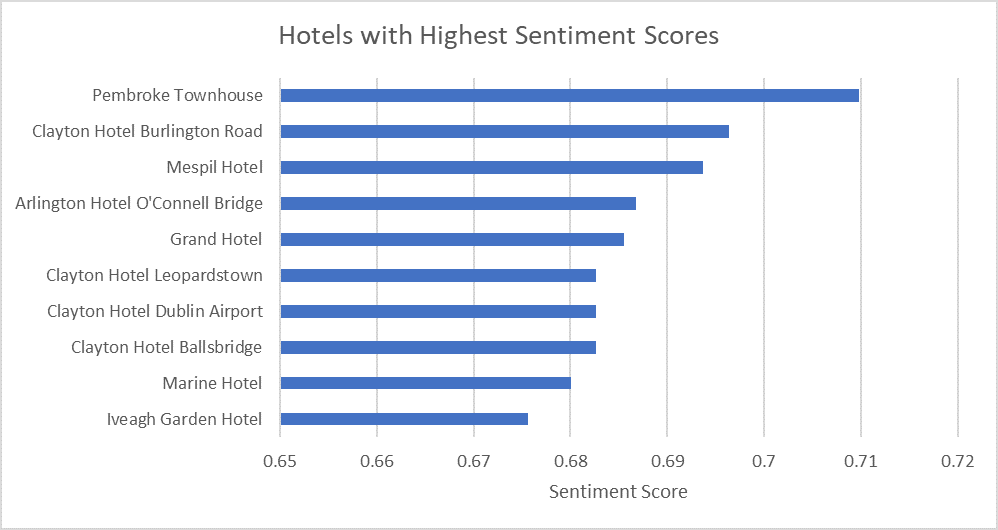
\includegraphics[width=1\textwidth]{evaluation/highest.png}
\caption{\label{fig:highest} Hotels with Highest Sentiment Scores.}
\end{figure}

\begin{figure}[h!]
\centering
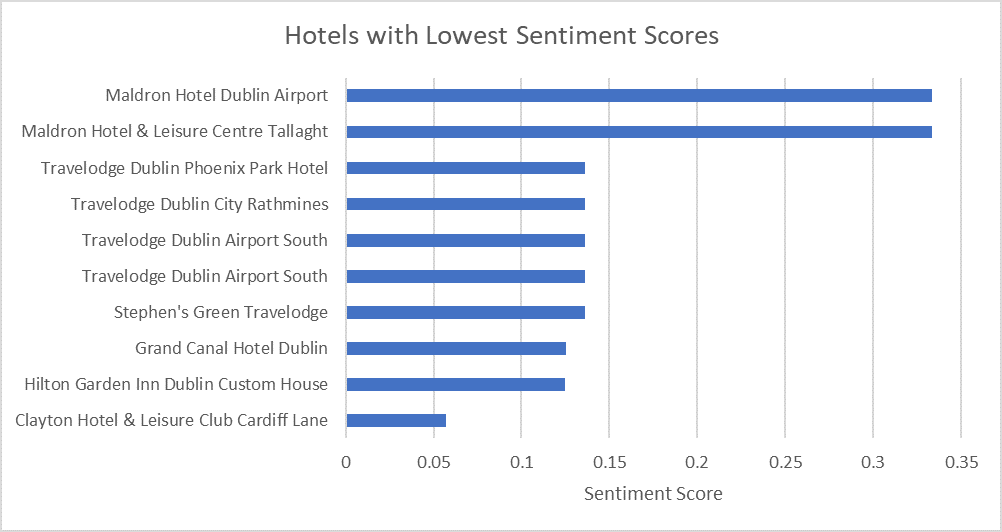
\includegraphics[width=1\textwidth]{evaluation/lowest.png}
\caption{\label{fig:lowest} Hotels with Lowest Sentiment Scores.}
\end{figure}

\section{Evaluation Metrics for Recommender Systems}

\subsection{CoRE Evaluation}

\subsubsection*{A/B Test}

A common evaluation for a recommender system is an A/B test. This is only possible if you have a recommender system with an existing user population. The test involves redirecting a percentage of the traffic to the new recommender system. The systems can then be compared based on implicit user feedback such as clicks and skips. An A/B test is currently being designed to incorporate CoRE into the live Ryanair Rooms website.

\subsubsection*{Leave-One-Out Cross Validation}

CoRE was evaluated using the 'leave-one-out' cross validation approach. In this approach one of a users n bookings is taken out and the remaining bookings are used to build the user model. A list of hotels is produced ranked in descending order by their predicted value. The booking that was removed is compared to this list to see where it ranked, the higher the better. This can be repeated with each of the users n bookings.

The Mean Percentile Rank (MPR) is then calculated.

\begin{equation}
    MPR = \frac{ \sum_{u,i} r_{ui} \times rank_{ui} } {\sum_{u,i} r_{ui}}
\end{equation}

$rank_{ui}$ is the percentile-ranking of hotel i within the ordered list of all hotels ranked for user u. $r_{ui}$ is a binary variable indicating whether user u booked hotel i. $rank_{ui} = 100\%$ indicates that the hotel i is predicted to be less desirable for user u. $rank_{ui} = 0\%$ indicates that the hotel i is predicted to be the most desirable hotel for user u. $rank_{ui} = 50\%$ would be expected for a list of randomly ranked hotels.

\subsection{Evaluation of Added Sentiment Scores}

This 'leave-one-out' approach was used to evaluate the CoRE recommender with the added sentiment scores. A four-way evaluation was carried out that compared the following:
\begin{enumerate}
    \item \textbf{Baseline} \newline
    The approach currently used by Ryanair in their rooms booking site.
    \item \textbf{CoRE} \newline
    The CoRE recommender system without the sentiment score added in.
    \item \textbf{Random} \newline
    A randomly ranked list of hotels.
    \item \textbf{Re-Ranked CoRE} \newline
    The CoRE recommender system re-ranked with the sentiment scores produced by the Stanford NLP Sentiment Analyser.
\end{enumerate}

\section{Recommender Results and Analysis}

\section{Summary}

\subsection{Classification}

One of the main aims of this research was to determine if it was possible to identify whether tweets contained reviews. A series of classifiers with different feature representations were implemented and evaluated. 

Overall considering the four classification metrics evaluated, the best performing classifier was the SVM Classifier, achieving the highest score in three out of four of the metrics, all but precision. The SVM classifier has a good balance of precision and recall, achieving the highest f1-score, and also had the highest accuracy score of all the classifiers.

A possible reason that SVM achieves the top performance is that the SVM classifier tends to be effective in high dimensional feature spaces. Twitter data produces a large feature set making this property of the SVM classifier useful. Another property of the SVM classifier is that they are still effective in cases where the number of dimensions is greater than the number of samples. The number of dimensions in this case is not higher than the number of samples. However our number of samples is relatively low.

\subsection{Recommender System}

The other aim of this research was to evaluate if review-like tweets could be used to appropriately influence the generation of recommendations in a recommender system. Sentiment scores were produced based on the classified tweets and used to re-rank the results of the CoRE recommender system. 

Incorporating the sentiment scores.... The effect of the sentiment scores was evaluated based on 21 hotels and 32 users. Ideally a larger test set is required to verify our results.

